\documentclass[12pt]{article}
\usepackage{amsmath}
\usepackage{subcaption}
\usepackage[utf8]{inputenc}
\usepackage{wrapfig}
\usepackage{float}
\usepackage{graphicx} % Required for inserting images
\usepackage{booktabs} % This and below for tables
\usepackage[breaklinks]{hyperref}
\hypersetup{colorlinks=true, linkcolor=Black, citecolor=Black, filecolor=Blue,
    urlcolor=Blue, unicode=true}
\usepackage[margin=1.2in]{geometry} % Adjust border

\renewcommand{\thesubsubsection}{(\alph{subsubsection})}


% For adding R code to appendix
\usepackage[T1]{fontenc}
\usepackage[latin1]{inputenc}

\usepackage{lmodern}% better font than default
\usepackage{tgcursor}% tt font with bold/italic styles

\usepackage{listings}
\lstset{
    language=R,
    basicstyle=\ttfamily
}


\begin{document}


\title{STA4026S Analytics - Neural Networks}

\author{Assignment 1\\
        Laurence Walton\\
        \href{mailto:wltlau003@myuct.ac.za}{wltlau003@myuct.ac.za}
}
\date{August, 2023}

\maketitle

\subsubsection{}
In the context of neural networks the soft-max activation function is used to turn an output layer into a probability distribution where each node has a value between 0 and 1 and the sum of the nodes is 1. This is relevant for multi-class classification problems because with soft-max applied each output node value can be treated as a probability where predictions may correspond to the node with the highest probability, and the error between the predicted probabilities and the true class labels can be used to adjust the network during the training process. The soft-max ensures that the predictions are scaled such that the error accurately reflects the disparities between the predicted probabilities.
The soft-max function in matrix form is:

\[
\sigma(z^n_j) = \frac{exp(z^n_j)}{\sum_{k=1}^q exp(z^n_k)}
\]

Where:
\begin{align*}
z^n_j & : \parbox[t]{0.7\textwidth}{The $j$-th node in the $n$-th training example, i.e. a value from the $q \times N$ output matrix where each row represents a node in the output layer and each column represents a training example} \\
\end{align*}

\subsubsection{}
A potential numerical pitfall in evaluating the cross-entropy error function arises if the predicted probability for a class is 0, as the evaluation would include the logarithm of 0 which is obviously undefined. This is mitigated by using activation functions such as the soft-max, where no predictions can be zero due to exponentiation. However, due to floating point imprecision in software, predictions could be rounded to zero in the soft-max, and therefore cause undefined behaviour in the cross-entropy error function.

\subsubsection{}

Plotting the cross-entropy error obtained on the validation data for varying values of $\nu$ yields the following curve, where I found the $\nu$ value of $0.09261443$ corresponds to the minimum error of $0.1259723$:

\begin{figure*}[!ht]
\centering
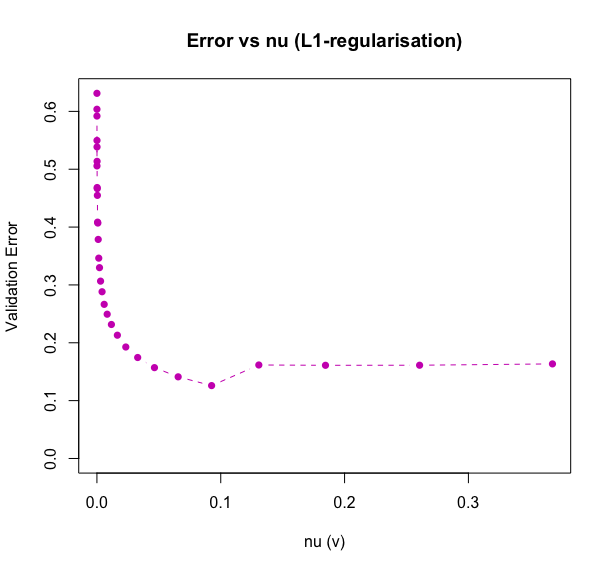
\includegraphics[width=0.8\textwidth]{question_c_plot.png}
\end{figure*}

\newpage
\subsubsection{}
Now I include use a new ANN which uses Rectified Linear Units (ReLU) as the hidden layer activation function. This is superimposed over the previous curve which showed an ANN using Tanh activation functions. I found the $\nu$ value of $0.09261443$ corresponds to the minimum error of $0.1207693$:

\begin{figure*}[!ht]
\centering
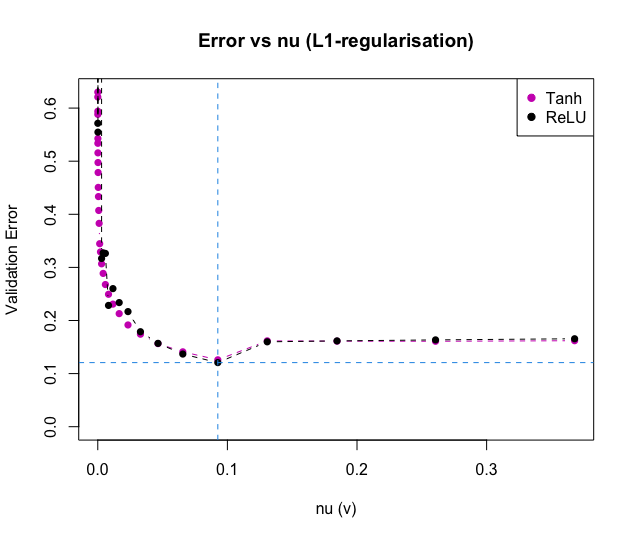
\includegraphics[width=0.8\textwidth]{question_d_plot.png}
\end{figure*}

\newpage

\subsubsection{}
Here I trained a neural network with tanh activation in the hidden layer on the complete data set, both with and without L1 regularization. Comparing the magnitude of the parameters between these two models provides insights into the model's complexity. L1 regularization introduces more 'sparsity', essentially reducing the effective number of parameters. In this case specifically, with L1 regularization, many of the model's parameters shrank to near-zero or zero and the largest parameter magnitudes were also reduced. The fact that the regularization promotes such strong sparsity indicates that the original model, without regularization, might have been overfitting the data, capturing excessive variance instead of the true underlying patterns. In simpler terms, the original model had high variance, which might have compromised its generalization capability on unseen data. The reduced number of effective parameters and reduced magnitudes show that the model can better perform on data outside of the training set.

 
\begin{figure*}[!ht]
\centering
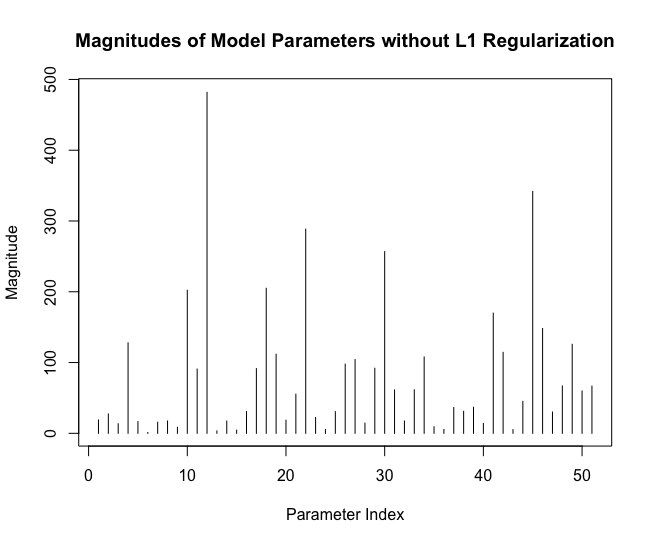
\includegraphics[width=0.5\textwidth]{question_e_plot_B.png}
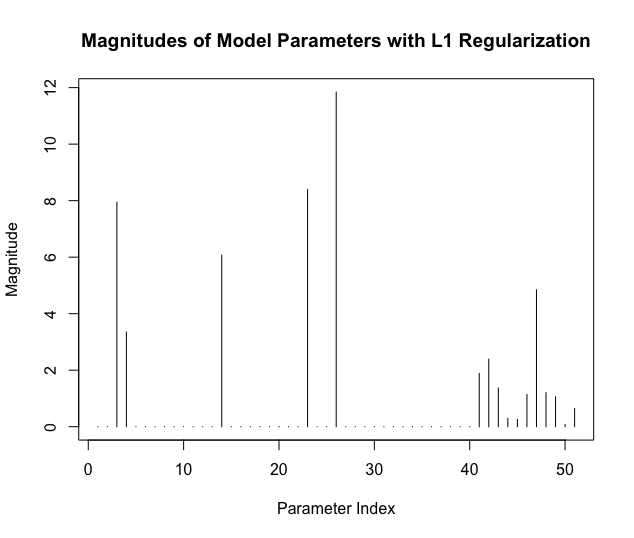
\includegraphics[width=0.5\textwidth]{question_e_plot_A.png}
\end{figure*}



\subsubsection{}
\begin{figure*}[!ht]
\centering
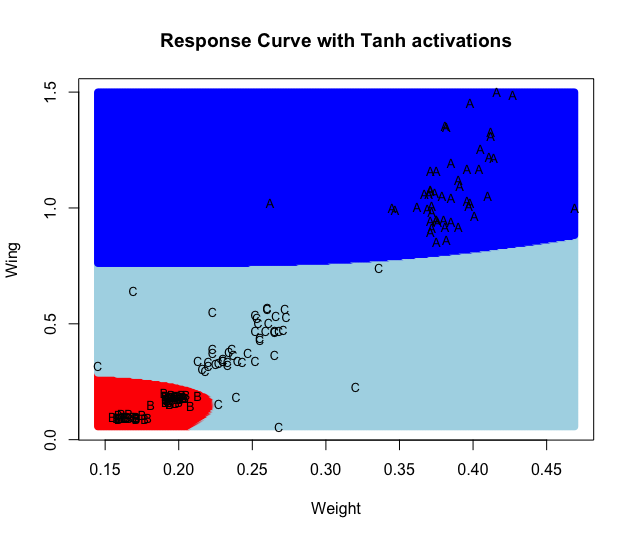
\includegraphics[width=0.7\textwidth]{question_f_plot_A.png}
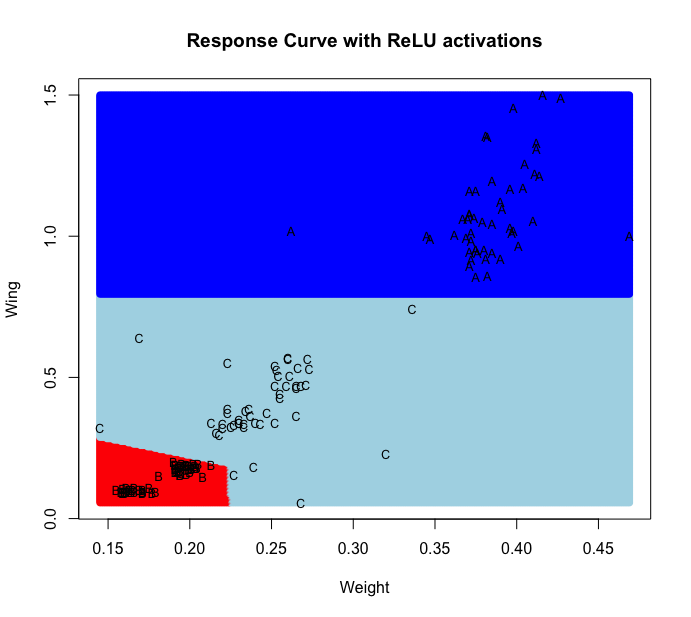
\includegraphics[width=0.7\textwidth]{question_f_plot_B.png}
\end{figure*}



\newpage
\appendix
\newgeometry{margin=0.1in}
\section{Appendix}
Raw R code from WLTLAU003\_Analytics\_A1.R:
\begin{lstlisting}
#
# (a)
#


# Function: softmax_matrix
# Description: Apply softmax to a matrix (N training examples)
#
# Arguments:
#   z_matrix: A q (no. nodes) X N (no. training examples) matrix
#
# Returns:
#   Matrix of same dim as z_matrix with softmax applied to each column
softmax_matrix <- function(z_matrix){
  
  softmax_vector = function(z){
    exp(z)/sum(exp(z))
  }
  
  res = matrix(0, nrow = dim(z_matrix)[1], ncol = dim(z_matrix)[2])
  for (j in 1:dim(z_matrix)[2]){  
    vec      = z_matrix[, j]        
    res[, j] = softmax_vector(vec)
  }
  return(res)
}


# Function: log_softmax_matrix
# Description: Apply log of softmax to a matrix (N training examples),
# avoiding over/under flow of values from normal softmax
#
# Arguments:
#   z_matrix: A p (no. features) X N (no. training examples) matrix
#
# Returns:
#   Matrix of same dimensions as z_matrix with log softmax applied 
#   to each column
log_softmax_matrix = function(z_matrix){
  
  log_softmax_vector = function(z){
    # Subtract the maximum value
    x = z - max(z)
    # Equation rearranging 
    log_softmax_z = x - log(sum(exp(x)))
    return(log_softmax_z)
  }
  
  # Apply the log_softmax_vector function to each column of z_matrix
  result_matrix = apply(z_matrix, 2, log_softmax_vector)
  
  return(result_matrix)
}


# (b)


# Function: tanh
# Description: Hyperbolic tangent function
tanh = function(z){
  # Do NOT use the bare calculation commented out - you may spend very
  # long thinking the softmax is causing over/under flow while it was 
  # tanh all along
  #(exp(z) - exp(-z))/(exp(z) + exp(-z))
  base::tanh(z)
}

# Function: neural_net
#
# Arguments:
#   X: Input matrix (N x p)
#   Y: Output matrix (N x q)
#   theta: A parameter vector (all of the parameters)
#   nu: Regularisation hyperparameter 
neural_net = function(X, Y, theta, nu)
{
  # Relevant dimensional variables:
  N     = dim(X)[1]
  p     = dim(X)[2]
  q     = dim(Y)[2]
  # Number of nodes (fixed at 8)
  m     = 8
  
  # Populate weight-matrix and bias vectors:
  index = 1:(p*m)
  W1    = matrix(theta[index], p, m) 
  index = max(index)+1:(m*q)
  W2    = matrix(theta[index], m, q)
  index = max(index)+1:(m)
  b1    = matrix(theta[index], m, 1)
  index = max(index)+1:(q)
  b2    = matrix(theta[index], q, 1)
  
  # Updating equations (matrix form)
  # mxN (8x148)
  b1    = matrix(rep(b1, N), nrow=m, ncol=N)
  
  # qxN (3x148)
  b2    = matrix(rep(b2, N), nrow=q, ncol = N)
  
  # pxN (2x148)
  a0    = matrix(t(X), p, N)

  # mxN (8x148)   
  a1    = apply(t(W1)%*%a0 +  b1, c(1,2), tanh)

  # qxN (3x148)        
  z2    = t(W2)%*%a1 + b2
  
  # softmax_matrix for when returning a2
  a2     = softmax_matrix(z2)
  # log_softmax_matrix for cross entropy calculation
  log_a2 = log_softmax_matrix(z2)
  
  # Cross-entropy error function for multi-class problems (q-dim) 
  cross_entropy <- -sum(t(Y) * log_a2)/N
  
  # Debugging
  #if (is.na(cross_entropy)){
  # browser()
  #}
  
  # Cross-entropy error with L1 penalty applied
  L1 <- cross_entropy + (nu/N * (sum(abs(W1)) + sum(abs(W2))))
                            
  # Return predictions and error:
  return(list(out=a2, cross_entropy=cross_entropy, L1=L1))
}


#
# (c)
#

set.seed(2023)

# Read in the data:
dat = read.table('Hawks_Data_2023.txt',h= T)
X   = as.matrix(dat[,4:5], ncol=2) 
Y   = as.matrix(dat[,1:3], ncol = 3)
N   = dim(dat)[1]

# Split data into training and test sets 
set = sample(1:N, 0.5*N, replace=FALSE)
X_train       = matrix(X[set,], ncol=2)
Y_train       = matrix(Y[set,], ncol = 3)

X_validation  = matrix(X[-set,], ncol=2)
Y_validation  = matrix(Y[-set,], ncol = 3)

# Return the error with L1 penalty applied when fitting
obj <- function(pars) {
  res <- neural_net(X_train, Y_train, pars, nu)
  return(res$L1)
}

# Network parameters
p = 2
q = 3
m = 8
npars = p*m+m*q+m+q

seq       = 30
val_error = rep(NA, seq)
lams      = exp(seq(-11, -1, length=seq))

for (i in 1:seq){
  nu      = lams[i]
  set.seed(2023)
  theta   = runif(npars,-1,1)
  res_opt = nlm(obj, theta, iterlim=1000)
  
  res_val = neural_net(X_validation, Y_validation, 
                       res_opt$estimate, 0) 
  
  val_error[i] = res_val$cross_entropy
  print(paste0('Val_Run_',i))
}


plot(val_error ~ lams, main = "Error vs nu (L1-regularisation)", 
     type = 'b', pch=16, lty=2, col = 6, lwd = 1, xlab = "nu (ν)", 
     ylab = "Validation Error", ylim=c(0,max(val_error)))

# Vertical line at the value of nu that has minimum val_error
abline(v=lams[which.min(val_error)], col=4, lty=2)
# Horizontal line at minimum val_error
abline(h=min(val_error), col=4, lty=2)
# Minimum validation error
min(val_error)
# Corresponding nu
lams[which.min(val_error)]


#
# (d)
#


# Function: ReLU
# Description: Apply ReLU to a vector (single training example). 
# Uses pmax(z,0) to apply the max-function element-wise
ReLU = function(z){
  pmax(z,0)
}

# Function: leaky_ReLU. 
# The parameter 'alpha' determines the slope for negative values, 
# allowing a small gradient when z is less than zero.
leaky_ReLU = function(z, alpha = 0.01){
  pmax(z, alpha * z)
}

# Function: neural_net_ReLU
# Description: Identical implementaion as question (b) but with 
# leaky ReLU activation for hidden layer
neural_net_ReLU = function(X, Y, theta, nu)
{
  # Relevant dimensional variables:
  N     = dim(X)[1]
  p     = dim(X)[2]
  q     = dim(Y)[2]
  # Number of nodes (fixed at 8)
  m     = 8
  
  # Populate weight-matrix and bias vectors:
  index = 1:(p*m)
  W1    = matrix(theta[index], p, m) 
  index = max(index)+1:(m*q)
  W2    = matrix(theta[index], m, q)
  index = max(index)+1:(m)
  b1    = matrix(theta[index], m, 1)
  index = max(index)+1:(q)
  b2    = matrix(theta[index], q, 1)
  
  # Updating equations (matrix form)
  # mxN (8x148)
  b1    = matrix(rep(b1, N), nrow=m, ncol=N)
  
  # qxN (3x148)
  b2    = matrix(rep(b2, N), nrow=q, ncol = N)
  
  # pxN (2x148)
  a0    = matrix(t(X), p, N)
  
  # mxN (8x148)   
  a1    = apply(t(W1)%*%a0 +  b1, c(1,2), leaky_ReLU)
  
  # qxN (3x148)        
  z2    = t(W2)%*%a1 + b2
  
  # Use log_softmax_matrix instead of softmax_matrix
  a2    = softmax_matrix(z2)
  log_a2 = log_softmax_matrix(z2)
  
  # Cross-entropy error function for multi-class problems (q-dim)
  cross_entropy <- -sum(t(Y) * log_a2)/N
  
  # Debugging
  if (is.na(cross_entropy)){
    browser()
  }
  # Cross-entropy error with L1 penalty applied
  L1 <- cross_entropy + nu/N * (sum(abs(W1)) + sum(abs(W2)))
  
  # Return predictions and error:
  return(list(out=a2, cross_entropy=cross_entropy, L1=L1))
}

# Return the error with L1 penalty applied when fitting,
# in this case use reLU NN
obj_ReLU <- function(pars) {
  res <- neural_net_ReLU(X_train, Y_train, pars, nu)
  return(res$L1)
}

# Network parameters
p = 2
q = 3
m = 8
npars = p*m+m*q+m+q

seq       = 30
val_error_ReLU = rep(NA, seq)
lams      = exp(seq(-11, -1, length.out=seq))

for (i in 1:seq){
  nu      = lams[i]
  set.seed(2023)
  theta   = runif(npars,-1,1)
  res_opt = nlm(obj_ReLU, theta, iterlim=1000)
  
  res_val_ReLU = neural_net_ReLU(X_validation, 
                                 Y_validation, res_opt$estimate, 0) 
  
  val_error_ReLU[i] = res_val_ReLU$cross_entropy
  print(paste0('Val_Run_',i))
}

# First plot the tanh (pink) line again 
# NOTE: must run loop in prev.question first to obtain val_error 
# Ensure all params the same (ie. iterlim, seq)
plot(val_error ~ lams, main = "Error vs nu (L1-regularisation)", 
     type = 'b', pch=16, lty=2, col = 6, lwd = 1, xlab = "nu (ν)", 
     ylab = "Validation Error", ylim=c(0,max(val_error)))

# Then superimpose the ReLU (black) line
lines(val_error_ReLU ~ lams, type = 'b', pch=16, lty=2, col=9, lwd=1)

# Legend, with Tanh first and then ReLU
legend("topright", col=c(6, 9), legend=c("Tanh", "ReLU"), pch=19)

# Vertical line at the value of nu that has minimum val_error
abline(v=lams[which.min(val_error_ReLU)], col=4, lty=2)

# Horizontal line at minimum val_error
abline(h=min(val_error_ReLU), col=4, lty=2)
# Minimum validation error
min(val_error_ReLU)
# Corresponding nu
lams[which.min(val_error_ReLU)]


#
# (e)
#


# Read in the data:
dat = read.table('Hawks_Data_2023.txt',h= T)
X   = as.matrix(dat[,4:5], ncol=2) 
Y   = as.matrix(dat[,1:3], ncol = 3)
N   = dim(dat)[1]

# Return the error with L1 penalty applied when fitting
obj_full_dataset <- function(pars) {
  res <- neural_net(X, Y, pars, nu)
  return(res$L1)
}

# Network parameters
p = 2
q = 3
m = 8
npars = p*m+m*q+m+q

nu = 0.09261443
theta   = runif(npars,-1,1)
res_opt = nlm(obj_full_dataset, theta, iterlim=1000)
optimal_pars <- res_opt$estimate

# Plot the magnitudes of the parameters with L1
plot(abs(optimal_pars), type = 'h', xlab = 'Parameter Index', 
     ylab = 'Magnitude', 
     main = 'Magnitudes of Model Parameters with L1 Regularization')

nu = 0
theta   = runif(npars,-1,1)
res_opt = nlm(obj_full_dataset, theta, iterlim=1000)
optimal_pars_no_reg <- res_opt$estimate

# Plot the magnitudes of the parameters without L1
plot(abs(optimal_pars_no_reg), type = 'h', xlab = 'Parameter Index', 
     ylab = 'Magnitude', 
     main = 'Magnitudes of Model Parameters without L1 Regularization')


#
# (f)
#


# Obtain the model trained on the full data set again
# Network parameters
p = 2
q = 3
m = 8
npars = p*m+m*q+m+q
nu    = 0.09261443
set.seed(2023)
theta   = runif(npars,-1,1)
res_opt = nlm(obj_full_dataset, theta, iterlim=1000)
optimal_pars <- res_opt$estimate

# Construct the plot for response curve
m = 300
wing_dummy       = seq(min(X[, "Wing"]), 
                       max(X[, "Wing"]), 
                       length=m)
weight_dummy     = seq(min(X[, "Weight"]), 
                       max(X[, "Weight"]), 
                       length=m)

plot (1, 1, type = 'n', xlim = range(X[, "Wing"]), 
      ylim = range(X[, "Weight"]),
      xlab="Wing", ylab="Weight")

abline(v=wing_dummy)
abline(h=weight_dummy)
x1 = rep(wing_dummy, m)
x2 = rep(weight_dummy, each=m)
points(x2~x1, pch=16)

# Use points on response curve to create a matrix 
# to be used for getting predictions
X_lattice = data.frame(Wing=x1, Weight=x2)
# The Y values are just zeros - not actually used when making these 
# predicitons as no error is being calculated, just getting the 
# outputs from the NN
m_zeros = rep(0,length=m)
y1 = rep(m_zeros, m)
y2 = rep(m_zeros, m)
y3 = rep(m_zeros, m)
Y_lattice = data.frame(SpecA=y1, SpecB=y2, SpecC=y3)

# Get predictions
res = neural_net(X_lattice, Y_lattice, optimal_pars, 0)
predictions = t(res$out)

# Obtain the class from each prediction by taking the highest 
# probability from softmax output
class = apply(predictions, 1, which.max)
cols = c('blue', 'red', 'lightblue')
plot(x2~x1, pch=16, col=cols[class], xlab="Weight", ylab="Wing", 
     main="Response Curve with Tanh activations")

# Plot the training data with a letter corresponding to the class 
numeric_to_char <- function(x) {
  return(LETTERS[x])
}
labels = apply(Y, 1, which.max)
char_labels = sapply(labels, numeric_to_char)
text(X[, "Weight"]~ X[, "Wing"], labels=char_labels, cex=0.8)



#
# (f) Part 2 (ReLU)
#

# Return the error with L1 penalty applied when fitting
obj_full_dataset_ReLU <- function(pars) {
  res <- neural_net_ReLU(X, Y, pars, nu)
  return(res$L1)
}

# Network parameters
p = 2
q = 3
m = 8
npars = p*m+m*q+m+q
nu = 0.09261443
set.seed(2023)
theta   = runif(npars,-1,1)
res_opt = nlm(obj_full_dataset_ReLU, theta, iterlim=1000)
optimal_pars <- res_opt$estimate

# Construct the plot for response curve
m = 300
wing_dummy       = seq(min(X[, "Wing"]), 
                       max(X[, "Wing"]), 
                       length=m)
weight_dummy     = seq(min(X[, "Weight"]), 
                       max(X[, "Weight"]), 
                       length=m)

plot (1, 1, type = 'n', xlim = range(X[, "Wing"]), 
      ylim = range(X[, "Weight"]),
      xlab="Wing", ylab="Weight")

abline(v=wing_dummy)
abline(h=weight_dummy)
x1 = rep(wing_dummy, m)
x2 = rep(weight_dummy, each=m)
points(x2~x1, pch=16)

# Use points on response curve to create a matrix 
# to be used for getting predictions
X_lattice = data.frame(Wing=x1, Weight=x2)
# The Y values are just zeros - not actually used when making these 
# predicitons as no error is being calculated, just getting the 
# outputs from the NN
m_zeros = rep(0,length=m)
y1 = rep(m_zeros, m)
y2 = rep(m_zeros, m)
y3 = rep(m_zeros, m)
Y_lattice = data.frame(SpecA=y1, SpecB=y2, SpecC=y3)

# Get predictions
res = neural_net_ReLU(X_lattice, Y_lattice, optimal_pars, 0)
predictions = t(res$out)

# Obtain the class from each prediction by taking the highest 
# probability from softmax output
class = apply(predictions, 1, which.max)
cols = c('blue', 'red', 'lightblue')
plot(x2~x1, pch=16, col=cols[class], xlab="Weight", 
     ylab="Wing", main="Response Curve with ReLU activations")

# Plot the training data with a letter corresponding to the class 
numeric_to_char <- function(x) {
  return(LETTERS[x])
}
labels = apply(Y, 1, which.max)
char_labels = sapply(labels, numeric_to_char)
text(X[, "Weight"]~ X[, "Wing"], labels=char_labels, cex=0.8)

\end{lstlisting}


\end{document}
